\section{Arendusmetoodika}

Käesolev jaotis kirjeldab arendusmetoodikat, mida töö teostamiseks rakendati.

\subsection{Hargnemismudel}

Arenduse tarbeks kasutatud versioonihalduse hargnemismudeliks valiti \textit{GitHub flow}. \textit{GitHub flow} taotleb arendamist ühel põhiharul, millesse mestitakse muudatusi lühikeste eluaegadega kõrvalharudest \cite{github-flow}. Samuti edendab \textit{GitHub flow} koodi läbivaatust enne harude mestimist \cite{github-flow}, mille hüvesid on kirjeldatud jaotises \ref{subsec:code-review}.

\subsection{Koodi läbivaatus}\label{subsec:code-review}

Koodi läbivaatus on tava, mille eesmärk on parandada ja säilitada koodi kvaliteeti \cite{gitlab-code-review}. Hea koodi läbivaatuse tulemusena on edasine arendus hõlpsam ning kliendile tarnimine turvakindlam \cite{gitlab-code-review}.

Koodi kvaliteedi tagamiseks ning vigade ilmumiste vähendamiseks otsustati arendusprotsessis läbi viia perioodilist koodi läbivaatust. Läbivaatust korraldati iga märkimisväärse muudatuse kohta ning seda viis läbi arendusest mitte osavõttev arendaja. Läbivaatuse käigus prooviti leida koodis loogikavigu ning leida viise kuidas protsesse selgemini väljendada. Lisaks koodiläbivaatustele viidi läbi arenduse käigus arutelusid, et lahendada keerulisemaid probleeme.

Koodi läbivaatust teostati GitHubi keskkonnas kasutades tõmbekutseid. Juhul kui arendused vajasid parandusi palus ülevaataja, et sinna tehtaks vajalikke muudatusi. Kui arendus sai heaks kiidetud mestiti see peaharuga.

\subsection{Tööjaotus}


\section{Vabavarasse panustamine}

Rakenduse arenduse käigus tuli ette olukordi, kus vabavaralised projekti sõltuvused vajasid kas täiendamist või parandamist, et töö saaks edukalt ning nõuetekohaselt jätkuda. Käesolev jaotis kirjeldab kordi, kui tarneahelas ülesvoolu tarkvaraprojektidesse oli otstarbekas muudatusi panustada.

\subsection{Teegi \emph{poetry2nix} hooldus}

Jaotises \ref{subsubsec:poetry2nix} mainitud \texttt{poetry2nix} teek paikab Nixpkgs arhiivist defineeritud Pythoni teeke, muutes nende tootestamissamme. Kuna Nixi paketihaldur taotleb korratavusgarantiisid, on sageli vaja tootestamiseks täpsustada kontrollsummasid.

Juhul, kui tootestamisprotsessis mõne sõltuvuse versioonid on uuenenud, ei saa Nixi paketihaldur neid üle võrgu alla tõmmata, kuna \texttt{poetry2nix} teegi paikadest puuduvad uuele versioonile vastavad kontrollsummad.

Kahel korral tekkis projekti tootestamisprotsessis sellise sündmuse tõttu viga. Joonistes \ref{fig:poetry2nix-patch1} ja \ref{fig:poetry2nix-patch2} on välja toodud paiked, mis parandasid eelmainitud vead, ning on nüüdseks \texttt{poetry2nix} teegi lähtekoodi mestitud \cite{poetry2nix-pr-1, poetry2nix-pr-2}.

\begin{figure}
\inputminted[breaklines]{diff}{chapters/data/poetry2nix-patch1.diff}
\caption{\emph{Poetry2nix teegi kontrollsumma paik nr 1.}}\label{fig:poetry2nix-patch1}
\end{figure}

\begin{figure}
\inputminted[breaklines]{diff}{chapters/data/poetry2nix-patch2.diff}
\caption{\emph{Poetry2nix teegi kontrollsumma paik nr 2.}}\label{fig:poetry2nix-patch2}
\end{figure}

\subsection{Teegi \textit{django-allauth} tõlkimine eesti keelde}

Pythoni teek \texttt{django-allauth} kaasab endaga palju tõlkeid \cite{django-allauth-i18n}, mida kasutatakse autentimisvoogudes kasutajale sõnumite edastamiseks. Enne bakalaureustöö alustamist ei toetanud \texttt{django-allauth} teek eesti keelt \cite{django-allauth-pre-et-i18n}.

Kuna üheks projekti nõuetest oli, et rakendus peab olema kättesaadav eesti keeles, siis oli otstarbekas panustada tõlked tarneahelas ülesvoolu poole, et vältida projekti lähtekoodis muudatuste haldamist. Teeki panustati pea täies mahus eestikeelsed tõlked \cite{django-allauth-et-i18n-pr}, mis on leida \texttt{.po} vormingus\footnote{\texttt{.po} failivorming on \texttt{GNU gettext} tööriistakomplektis defineeritud failivorming, mis on mõeldud tõlgete defineerimiseks. Failivorming on mõeldud olema kergesti mõistetav ka tõlkidele \cite{gnu-gettext-po}.} lisast ``\nameref{app:allauth-translations}''.

\subsection{Teegi \textit{django-allauth} Nix tarkvarapaketi parandused}\label{subsec:compile-mo}

Django projektid kasutavad tõlgete toetamiseks \texttt{GNU gettext} tööriistakomplekti \cite{django-gettext}. Tõlgete toimimiseks peab \texttt{.po} vormingus lihttekstfailid kompileerima \texttt{.mo} vormingus kahendfailideks \cite{django-gettext}.

Nixpkgs arhiivi kommete järgi eelistatakse võimaluse korral tootestada tarkvarapakette otse lähtekoodist. Django ja muude Django peale ehitatud teekide puhul tähendab see seda, et pakendamisel pakendatakse kaasa \texttt{.mo} kahendfailid, kuna neid hoitakse ülesvoolu projekti repositooriumites. Teegi \texttt{django-allauth} puhul aga puuduvad lähtekoodis \texttt{.mo} kahendfailid — need pakendatakse kaasa eraldi tootestamissammus PyPI paketiarhiivi väljalaset tarnides \cite{django-allauth-no-mo-files}.

Kokkuvõttes tähendab see seda, et teegi \texttt{django-allauth} tõlked töötavad vaikimisi, kui teek on paigaldatud \texttt{pip install}\footnote{\texttt{pip} on ametlikult soovitatud tööriist PyPI arhiivist Pythoni teekide paigaldamiseks \cite{pip-standard}} käsu või mõne muu PyPI arhiivist teeke paigaldava käsuga, ent mitte Nixi paketihalduriga pakendatud Pythoni projektis.

Olukorra leevendamiseks sooritati Nixpkgs arhiivi repositooriumisse tõmbekutse, mis vea parandas \cite{nixpkgs-compile-mo}. Nixi tarkvarapaketi definitsiooni paik on kirjeldatud joonises \ref{fig:compile-mo-patch}. Kirjutamise ajal pole tõmbekutse sisu repositooriumisse mestitud. 

\begin{figure}
\inputminted[breaklines]{diff}{chapters/data/compile-mo.diff}
\caption{\emph{Teegi \texttt{django-allauth} Nix tarkvarapaketti parandav paik.}}\label{fig:compile-mo-patch}
\end{figure}

\subsection{Teegi \textit{dj-rest-auth} testide hooldused}

Jaotises \ref{subsec:compile-mo} kirjeldatud parandusi ellu viies oli otstarbekas ka juba tarkvarapaketi versiooni uuendada. Autorid tegid tõmbekutse Nixpkgs paketiarhiivi repositooriumisse \cite{allauth-bump-nixpkgs}, mis uuendas eelmainitut versioonilt \texttt{0.61.1} versioonile \texttt{0.62.0}.

Kuna Nixi paketihaldur ei toeta tarkvarapakettide versioonide lahendamist ja haldamist\footnote{Nixi jaoks on paketi identiteet täielikult tootestamissammudele antud sisendite kontrollsummadest määratud \cite{nixos-how-nix-works} — \texttt{(pakett-A, v1.0.0)} ning \texttt{(pakett-A, v1.0.1)} on täiesti üksteisest eristamatud. Sellegipoolest on versioonilahendus oluline, ning seda taasimplementeeritakse paketiarhiivi lähtekoodis \cite{python3-nix-versioning}.}, võivad tekkida iga uue versioonihalduse \emph{commit}'i puhul lahkhelid sõltuvusgraafis.

Selline lahkheli tekkis versiooni uuendamisel: repositooriumis oli tarkvarapakett, mille testid sõltusid \texttt{django-allauth} teegist \cite{test-dep} — selle testid lakkasid edukalt jooksmast, kuna uues \texttt{django-allauth} versioonis oli teegi sisemusi ringi liigutatud ning ümber kirjutatud.

Vea parandamiseks avasid autorid tõmbekutse tarneahelas ülesvoolu projektis \texttt{dj-rest-auth}, mis parandas teste niiviisi, et nad töötaksid ka uue \texttt{django-allauth} versiooniga \cite{dj-rest-pr}.

\subsection{Hunspell sõnastiku Nix pakendi loomine}

Hunspell on õigekirjakontrolli teostav programm, mida kasutavad Google Chrome, Mozilla Firefox, macOS, LibreOffice ja Thunderbird \cite{hunspell}.
Käesoleval bakalaureusetööl õigekirjakontrolli arenduskeskkonnas ja pidevas integratsioonis rakendamise tarbeks pakendasid autorid Hunspellile eestikeelsed sõnastikud \cite{hunspell-pr}. Nixpkgs arhiivi tehtud tõmbekutse sisu kirjeldab joonis \ref{fig:hunspell-pr}.

\begin{figure}[H]
\inputminted[breaklines]{diff}{chapters/data/hunspell.diff}
\caption{\emph{Nixpkgs arhiivi Hunspelli eestikeelse sõnastiku paki lisamine.}}\label{fig:hunspell-pr}
\end{figure}

\section{Rakenduse arendus}

\subsection{Ülesannete genereerimine}

Ülesannete genereerimiseks vajas iga ülesandetüüp eraldi implementatsiooni. Selle teostamiseks määrati igale ülesandetüübile üldkuju, milles olid kindlates asukohtades muutujad. Erinevate ülesannete saamiseks kasutati suvaliselt genereeritud numbreid, mis täitsid muutujate väärtused.

Paraku on sellist meetodit kasutades suur probleem vastuste kujudega. Kuna suvalisi numbreid kasutades on ebatõenäoline, et vastus taandub väiksemale kujule, on tihti vastuste väärtused pikad ning ebamugavad arvutamiseks ilma kalkulaatorita. Probleemi parandamiseks on võimalik piirata kasutatavate suvaliste numbrite hulka ning vältida suuremaid numbreid täiesti. Selle tulemusena on võimalike ülesannete hulk palju väiksem, kuid ikkagi piisavalt suur, et korduvate ülesannete ilmumine ei oleks tõenäoline.

Peale ülesande definitsiooni koostamist arvutatakse automaatselt probleemi vastus kasutades SymPy teeki. Arenduse käigus avastati, et SymPy ei kuva alati võrratusi samamoodi ning lisab mõnele muutujale juurde ühega korrutamise. Korrutamise erisus ei muuda vastuse väärtust ega lahendamise protsessi, kuid on nähtav probleemi definitsioonis. Töö kirjutamise ajal ei lahendatud seda probleemi, kuna see ei langenud kokku süsteemi nõuetega (vaata jaotis \ref{sec:nonfunctional-requirements}). Joonis \ref{fig:maths} kuvab ruutvõrratuste loomise lähtekoodi.

Rakendus toetab kolme ülesandetüüpi:
\begin{itemize}
  \item lineaarvõrratusi
  \item ruutvõrratusi
  \item murdvõrratusi
\end{itemize}

\begin{figure}
\inputminted[breaklines]{py}{chapters/data/maths.py}
\caption{\emph{Ruutvõrratuse loomise lähtekood.}}\label{fig:maths}
\end{figure}

\subsection{Andmemudelite loomine}

\subsubsection{Olemisuhtediagramm}

Joonises \ref{fig:uml} on näidatud rakenduse lihtsustatud olemisuhtediagramm.

\begin{figure}
\begin{adjustbox}{width=\textwidth}
\includesvg{chapters/data/uml.svg}
\end{adjustbox}
\caption{\emph{Rakenduse olemisuhtediagramm.}}\label{fig:uml}
\end{figure}

\subsection{Vaadete loomine}

Töö nõuete täitmiseks oli vajalik luua mitu vaadet, mis tagaks kasutajale võimaluse luua ning hallata teste ja testide malle (vt jaotis \ref{sec:functional-requirements}).

Rakendusele loodi järgnevad vaated:
\begin{itemize}
  \item sisselogimise vaade
  \item konto loomise vaade
  \item rakenduse koondpaneel ehk avalehe vaade
  \item mallide koondvaade
  \item malli loomise vaade
  \item malli detailvaade
  \item malli detailide uuendamise vaade
  \item malli probleemi lisamise vaade
  \item malli probleemi uuendamise vaade
  \item testi genereerimise vaade
  \item testi salvestamise vaade
  \item testide koondvaade
  \item testi detailvaade
  \item ülesande tüüpide koondvaade
  \item ülesande variandi alla laadimise vaade
  \item ülesande vastustelehe alla laadimise vaade
\end{itemize}

Joonis \ref{fig:dashboard_view} kuvab rakenduse avalehte. Joonis \ref{fig:template_details_view} kuvab malli detailvaadet. Joonis \ref{fig:test_generation_save_view} kuvab testi salvestamise vaadet peale seda kui test on genereeritud.

Rakenduse esmasel kasutusel saabub kasutaja sisselogimise vaatele. Sealt edasi on tal võimalik täita kasutajanime ja salasõna väljad ning rakendusse sisse logida.

\begin{figure}[H]
    \centering
    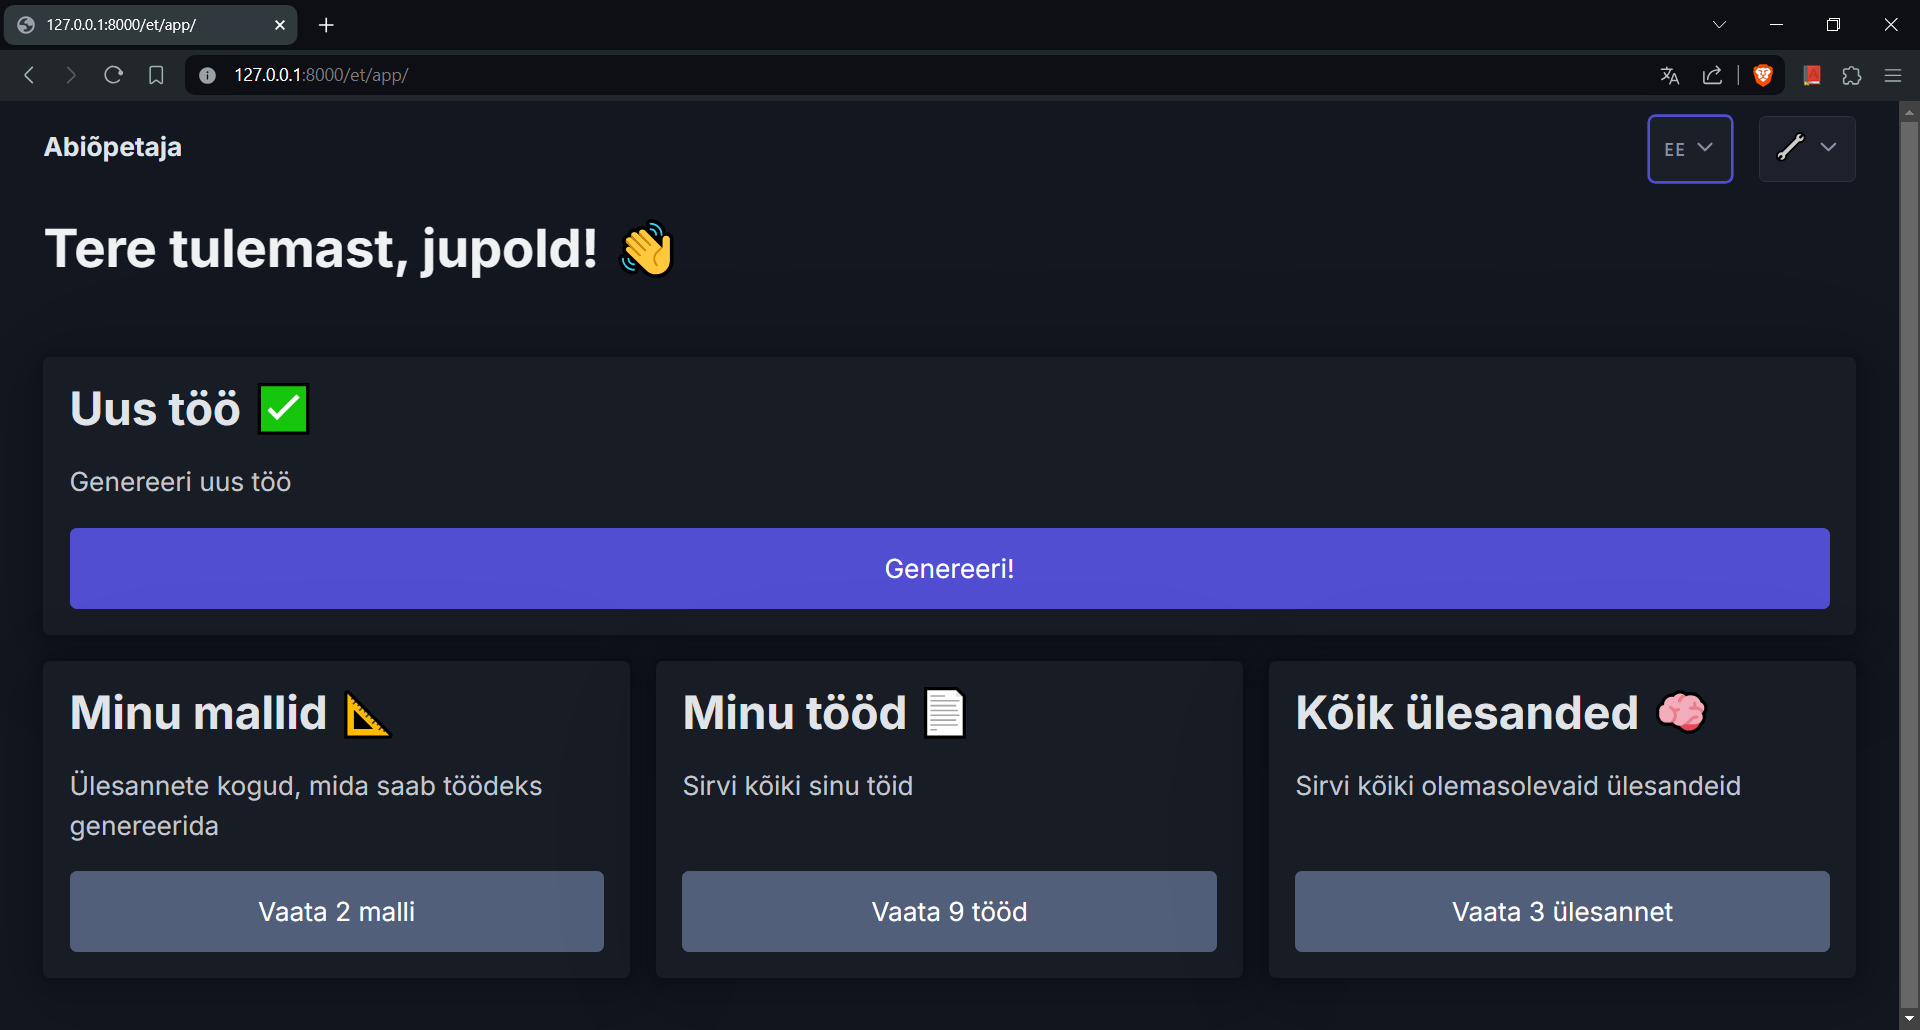
\includegraphics[width=\textwidth]{dashboard_view}
    \caption{Rakenduse avalehe vaade}
    \label{fig:dashboard_view}
\end{figure}

\begin{figure}[H]
    \centering
    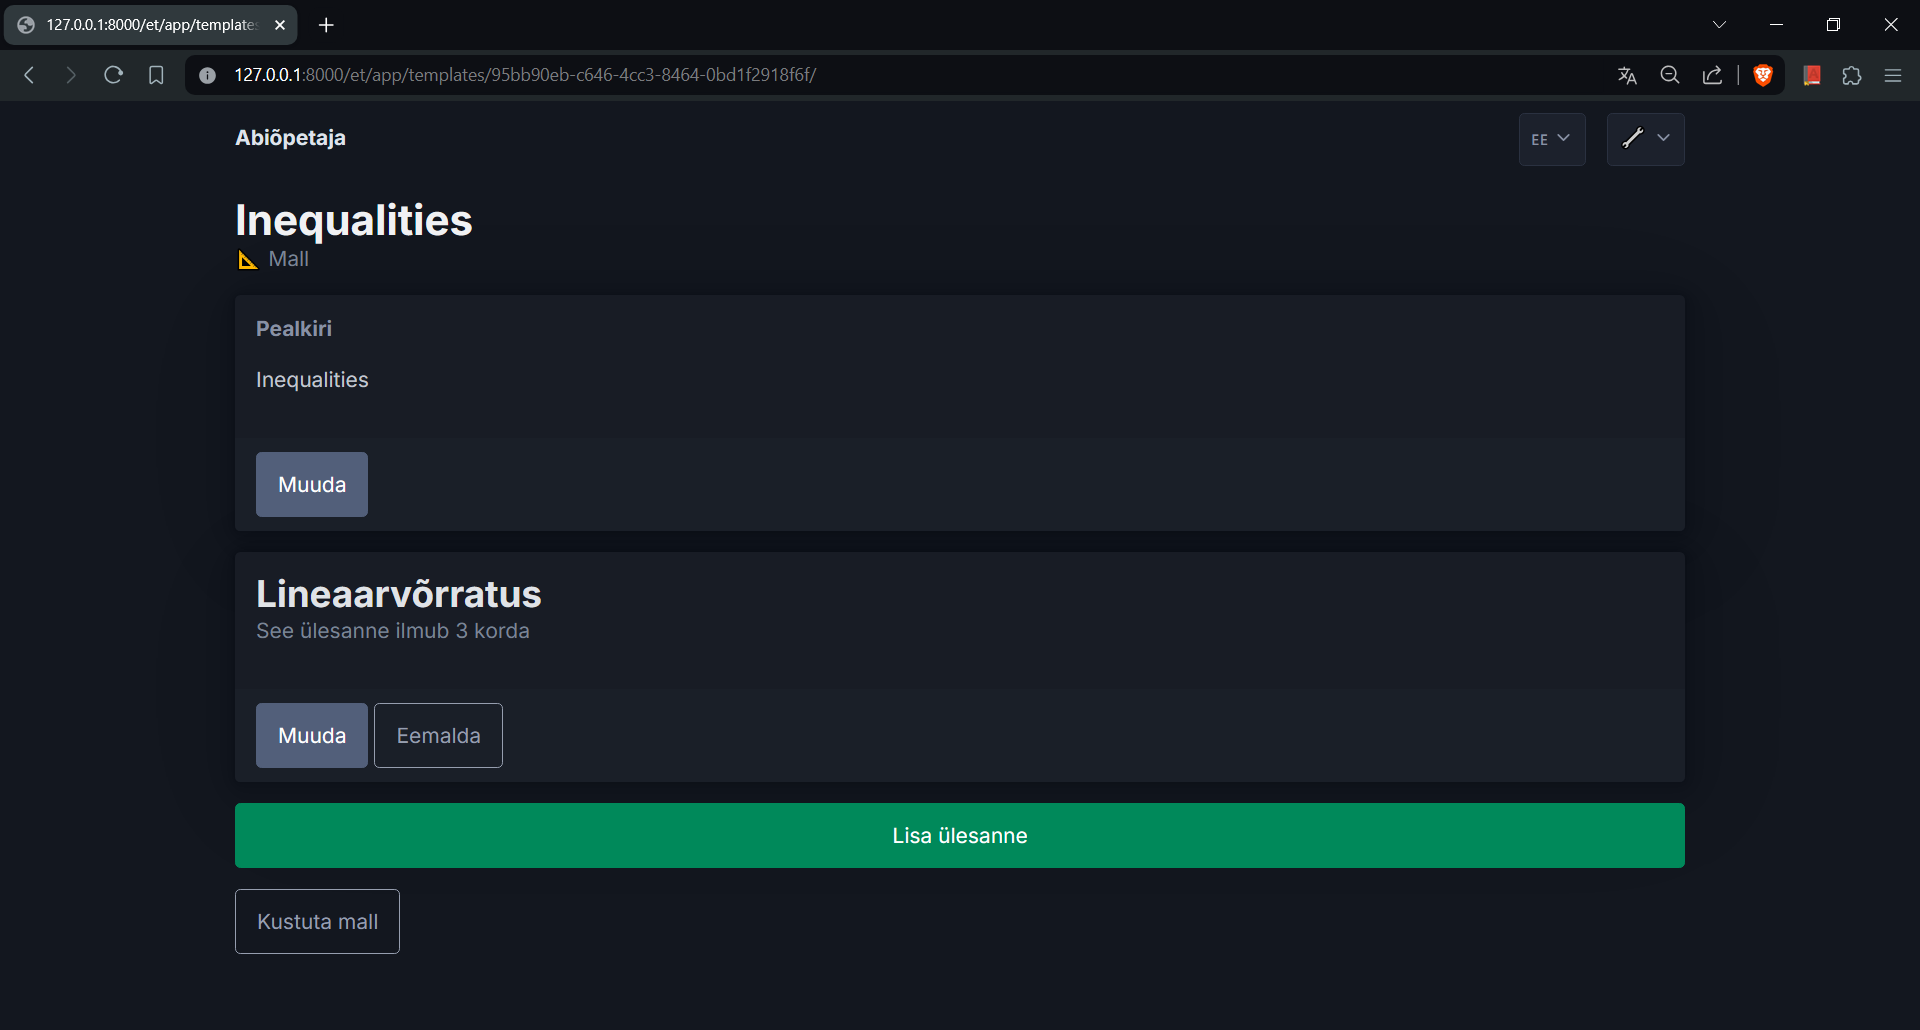
\includegraphics[width=\textwidth]{templates_details_view}
    \caption{Malli detailvaade}
    \label{fig:template_details_view}
\end{figure}

\begin{figure}[H]
    \centering
    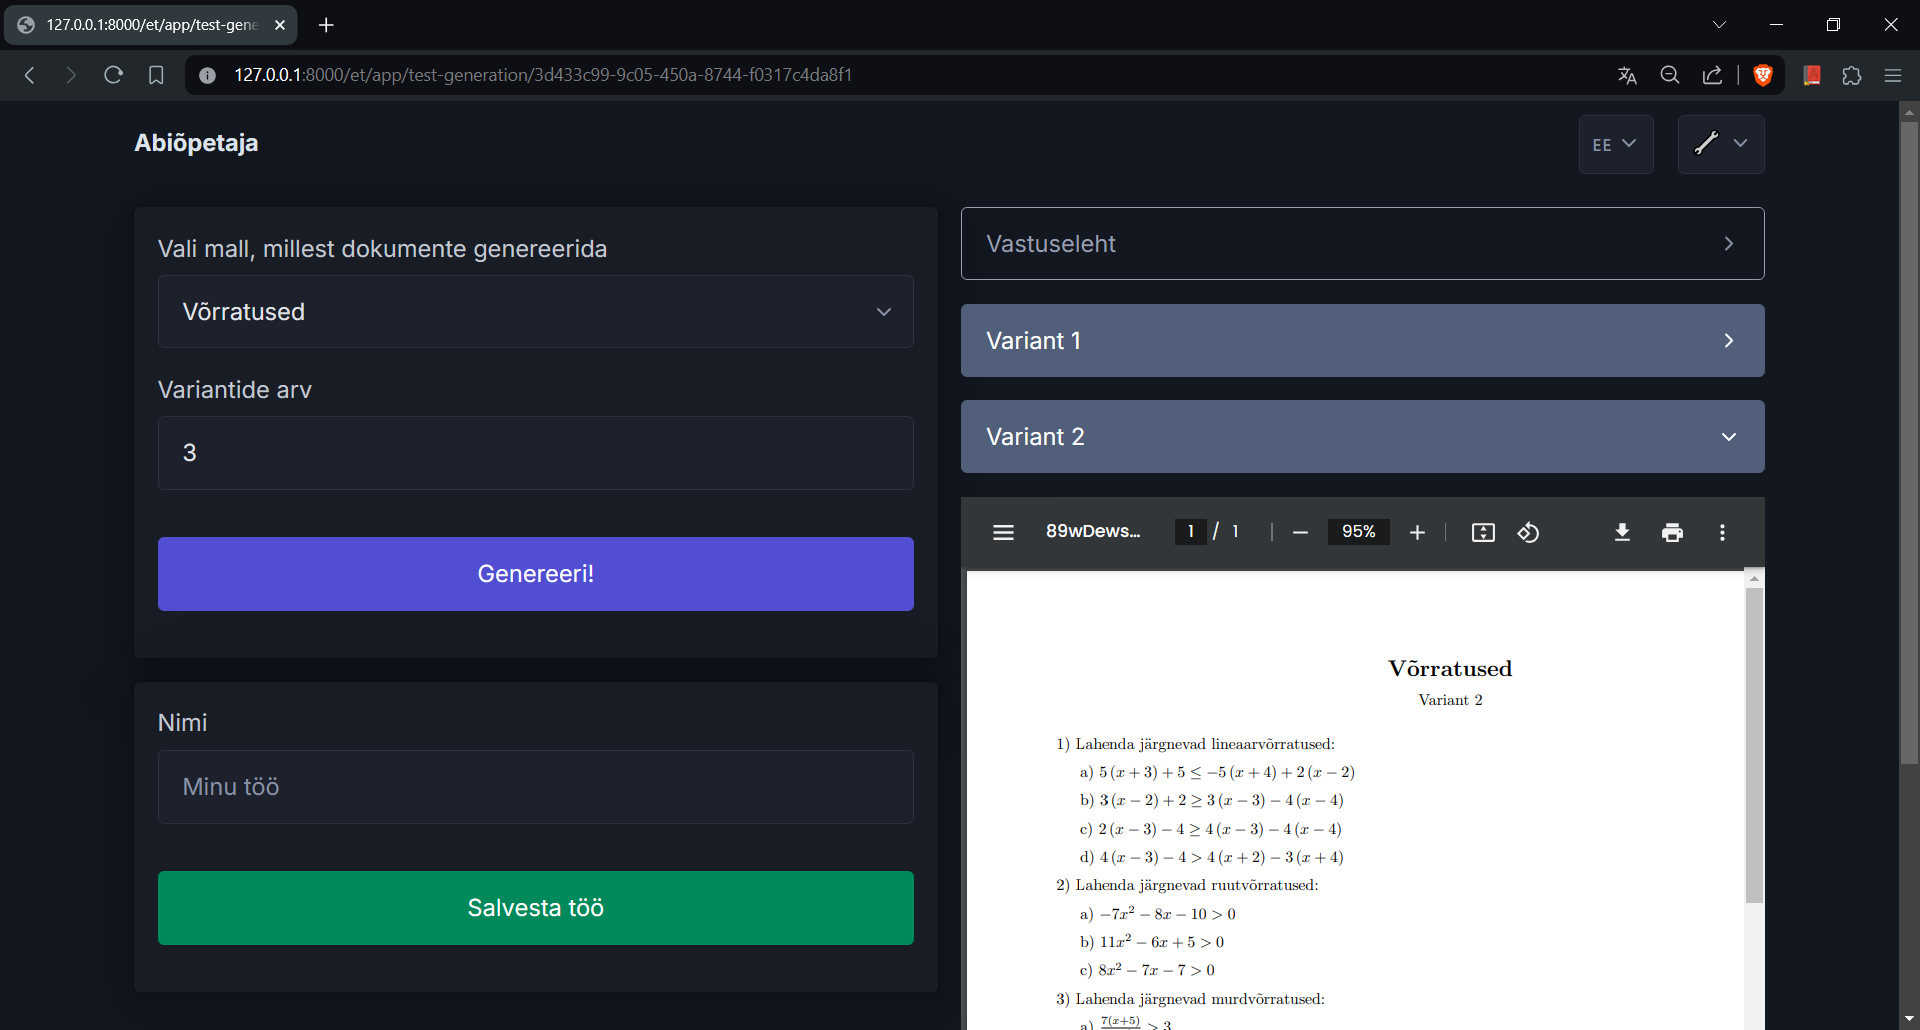
\includegraphics[width=\textwidth]{test_generation_save_view}
    \caption{Testi salvestamise vaade}
    \label{fig:test_generation_save_view}
\end{figure}

\subsection{Rakenduse testimine}

Tagamaks rakenduse testituse nõuet (vt jaotis \ref{sec:nonfunctional-requirements}) kirjutati rakendusele nii Django raamistiku testimisliidestele \cite{django-testing-api} tuginevad integratsioonitestid, kui ka virtuaalmasinavõrkudes jooksvad NixOS testid \cite{nixos-tests} (vt jaotist \ref{subsubsec:e2etests}).

\subsubsection{Integratsioonide testimine}

Veebiraamistiku tasemel rakenduse erinevate kihtide integratsioonide testimiseks kasutati \texttt{pytest-django} teeki, mis võimaldab
\texttt{pytest} testimisraamistiku kaudu kutsuda Django raamistiku testimisliideseid \cite{pytest-django-usage}. Teegi \texttt{pytest} testide jooksutamise tulemusena on testimiskood oluliselt kompaktsem ja kergemini loetav \cite{pytest-django-why}.

Joonis \ref{fig:pytest} kuvab katkendit lähtekoodi testimismooduli lähtekoodist.

\begin{figure}
\inputminted[breaklines]{py}{chapters/data/test.py}
\caption{\emph{Üks testimismooduli integratsioonitestidest.}}\label{fig:pytest}
\end{figure}

\subsubsection{Läbivtestimine}\label{subsubsec:e2etests}

\newcommand{\stateActually}{Tegelikkuses kirjeldavad NixOS konfiguratsioonid paketi tootestamisel toodetuid skripte ja muid ressursse, mis hostile NixOS konfiguratsiooni paigaldavad. Praktikas on tööriistakomplekti korratavusgarantiid nii tugevad, et sellest võib mõelda kui konfiguratsiooni olekust hostil.}

Läbivtestimise eelduseks on NixOS mooduli defineerimine, mis kirjeldab Abiõpetaja rakenduse paigaldust NixOS operatsioonisüsteemis. Mooduli abil on edaspidi võimalik realiseerida NixOS konfiguratsioone \cite{nixos-configuration}, mis kirjeldavad operatsioonisüsteemi olekut\footnote{\stateActually} läbivtestimiskeskkonnas või tarbekeskkonnas. Abiõpetaja rakenduse paigaldust kirjeldav NixOS moodul on välja toodud lisas ``\nameref{app:nixosmodule}''.

Moodulit saab kasutada virtuaalmasinatestide defineerimiseks. Joonis \ref{fig:test-vm-server} kirjeldab virtualiseeritud läbivtestimiskeskkonnas rakenduse serveri hosti konfiguratsiooni. Joonis \ref{fig:vm-tests} kirjeldab läbivteste, mida pidevas integratsioonis jooksutatakse (vt jaotis \ref{subsec:cicd}).

Oluline on märkida, et tarbekeskkonna rakenduse konfiguratsioon (vt jaotis \ref{subsec:cicd}) erineb vaid väärtuste \texttt{provisionCertificates} ning \texttt{domains} poolest, mis tähendab, et läbivtestkeskkond on tarbekeskkonnale nõuetekohaselt (vt jaotis \ref{sec:nonfunctional-requirements}) maksimaalselt sarnane.

\begin{figure}
\inputminted[breaklines]{nix}{chapters/data/test-vm-server.nix}
\caption{\emph{Läbivtestkeskkonnas kasutatava serveri hosti NixOS konfiguratsioon.}}\label{fig:test-vm-server}
\end{figure}

\begin{figure}
\inputminted[breaklines]{nix}{chapters/data/vm-tests.nix}
\caption{\emph{Nix programmeerimiskeele funktsioon, mis tagastab järjendi läbivtestidega.}}\label{fig:vm-tests}
\end{figure}

\subsection{Rakenduse tarnimine}\label{subsec:cicd}

Käesolev jaotis kirjeldab rakenduse tarnimist.

\subsubsection{Taristu hankimine}

Rakenduse tarnimiseks vajalikku ning jaotises \ref{subsec:ec2} kirjeldatud Amazon EC2 virtuaalmasina hankimiseks kasutati jaotises \ref{subsec:opentofu} kirjeldatud OpenTofu tööriista. Taristu definitsiooni \texttt{.tf} vormingus on loetletud lisas ``\nameref{app:infra}''.

\subsubsection{CI/CD konveier}

Nõuetekohase pidevat integratsiooni (vt jaotist \ref{sec:nonfunctional-requirements}) tagamiseks defineeriti Nixi tarkvarapaketid, mida GitHub Actions konveieris tootestati.

Joonis \ref{fig:ci-yaml} kirjeldab \texttt{.yaml} vormingus GitHub Actions tööplaani, mis seab üles Nixi paketihalduriga keskkonna ning jooksutab tarkvarapakettides defineerituid teste ja kvaliteedikontrolle.

\begin{figure}
\inputminted[breaklines]{yaml}{chapters/data/ci.yaml}
\caption{\emph{GitHub Actions tööplaan pidevaks integratsiooniks.}}\label{fig:ci-yaml}
\end{figure}

Pideva tarnimise teostamiseks kasutati jaotises \ref{subsubsec:deploy-rs} kirjeldatud tööriista \texttt{deploy-rs}. Joonis \ref{fig:deploy-rs-config} kirjeldab \texttt{deploy-rs} programmile antud tarnimiskonfiguratsiooni. Tarnimiskonfiguratsiooni jaoks vajalik avalik IP aadress on võetud OpenTofu taristu üles seadmise väljundist.

\begin{figure}
\inputminted[breaklines]{nix}{chapters/data/deploys.nix}
\caption{\emph{Programmile \texttt{deploy-rs} edastatud konfiguratsioon.}}\label{fig:deploy-rs-config}
\end{figure}

Eelnevalt hangitud virtuaalmasinale tarniti joonises \ref{fig:ec2-config} kirjeldatud NixOS konfiguratsioon. 

\begin{figure}
\inputminted[breaklines]{nix}{chapters/data/ec2-config.nix}
\caption{\emph{Virtuaalmasinale tarnitud NixOS konfiguratsioon.}}\label{fig:ec2-config}
\end{figure}

Joonis \ref{fig:cd-yaml} kirjeldab \texttt{.yaml} vormingus GitHub Actions tööplaani, mis seab üles Nixi paketihalduriga keskkonna ning tarnib NixOS konfiguratsiooni eelnevalt hangitud virtuaalmasinale.

\begin{figure}
\inputminted[breaklines]{yaml}{chapters/data/cd.yaml}
\caption{\emph{GitHub Actions tööplaan pidevaks tarnimiseks.}}\label{fig:cd-yaml}
\end{figure}

